\documentclass[12pt, a4paper]{article}

\usepackage[
  margin=1in
]{geometry}

\usepackage[T1, T2A]{fontenc}
\usepackage[utf8]{inputenc}
\usepackage[russian]{babel}
\usepackage{minted}
\usepackage{hyperref}
\usepackage{tabularray}
\usepackage{amsmath,amssymb}
\usepackage{float}
\usepackage{graphicx}
\usepackage{multicol}

\graphicspath{ {./img/} }

\begin{document}

\begin{titlepage}
  \centering
  \textsc{Новосибирский государственный технический университет}\par
  \vspace{1mm}
  Кафедра теоретической и прикладной информатики\par
  \vspace{8cm}
  \textsc{Расчётно-графическая работа}\par
  {\huge\bfseries Математическая статистика\par}
  \vspace{1cm}
  {\scriptsize ФПМИ, ПМ-24, В17\par}
  \vspace{1mm}
  {\itshape\large Параскун И.\par}
  \vfill
  {\small преподаватели\par}
  \vspace{2mm}
  \textsc{Тимофеева А. Ю.}\par
  \vspace{1mm}
  \textsc{Кутузова И. А.}\par
  \vfill
  \large{Новосибирск, 2024}
\end{titlepage}

\newpage
\setcounter{page}{2}

\section{Часть 1}
\subsection{Постановка задачи}
Дана следующая выборка из генеральной совокупности:

\begin{align*}
  X = \left[ 
    9.4, 7.3, 9.4, 8.4, 8.7, 5.7, 6.3, 5.3, 
    -1.2, 5.2, 3.6, 4.3, 11.5, 6.5, 8.2 
  \right]
\end{align*}

\vspace{3mm}

\noindent Учитывая, что $\gamma = 0.95$, $a = 7$, $\sigma = 3$, выполнить следующие
задания:

\begin{enumerate}
  \item Построить график эмпирической функции распределения. 
    Построить график функции распределения;
  \item Найти оценку математического ожидания, несмещенные оценки 
    дисперсии при известном и неизвестном математическом ожидании;
  \item Построить доверительные интервалы для математического ожидания 
    и стандартного отклонения при известном и неизвестном втором параметре 
    соответственно.
\end{enumerate}

\subsection{Ход выполнения}

\begin{table}[H]
\centering
\begin{tblr}{
  width=\textwidth, 
  colspec={|X|X|X|X|X|X|X|},
  rowspec={|c|cccccccccccccc|c|}
}
\SetCell{c} $x_i$ & \SetCell{c} $n_i$ & \SetCell{c} $p_i$ & \SetCell{c} $x_ip_i$ & \SetCell{c} $F^*(x_i)$ & \SetCell{c} $p_i(x-a)^2$  & \SetCell{c} $p_i(x-\bar{X})^2$  \\
-1.2	            & 1	                & 0.067	            & -0.080	             & 0.067	                & 4.483	                    & 4.028                           \\
3.6	              & 1	                & 0.067	            & 0.240	               & 0.133	                & 0.771	                    & 0.589                           \\
4.3	              & 1	                & 0.067	            & 0.287	               & 0.200	                & 0.486	                    & 0.345                           \\
5.2	              & 1	                & 0.067	            & 0.347	               & 0.267	                & 0.216	                    & 0.126                           \\
5.3	              & 1	                & 0.067	            & 0.353	               & 0.333	                & 0.193	                    & 0.108                           \\
5.7	              & 1	                & 0.067	            & 0.380	               & 0.400	                & 0.113	                    & 0.051                           \\
6.3	              & 1	                & 0.067	            & 0.420	               & 0.467	                & 0.033	                    & 0.005                           \\
6.5	              & 1	                & 0.067	            & 0.433	               & 0.533	                & 0.017	                    & 0.000                           \\
7.3	              & 1	                & 0.067	            & 0.487	               & 0.600	                & 0.006	                    & 0.035                           \\
8.2	              & 1	                & 0.067	            & 0.547	               & 0.667	                & 0.096	                    & 0.176                           \\
8.4	              & 1	                & 0.067	            & 0.560	               & 0.733	                & 0.131	                    & 0.222                           \\
8.7	              & 1	                & 0.067	            & 0.580	               & 0.800	                & 0.193	                    & 0.302                           \\
9.4	              & 2	                & 0.133	            & 1.253	               & 0.933	                & 0.768	                    & 1.065                           \\
11.5	            & 1	                & 0.067	            & 0.767	               & 1.000	                & 1.350	                    & 1.618                           \\
$\Sigma$          & 15                & -                 & 6.573                & -                      & 8.853                     & 8.671
\end{tblr}
\caption{Дискретный вариационный ряд}
\end{table}

\begin{figure}[H]
\centering
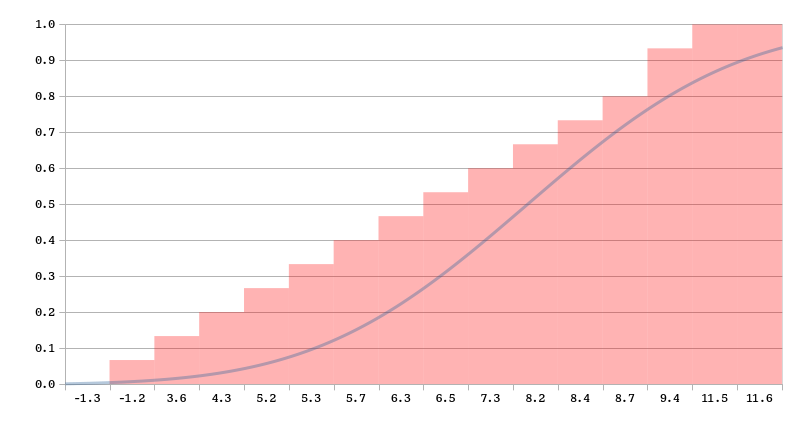
\includegraphics[scale=0.55]{1.png}
\caption{Эмпирическая функция распределения}
\end{figure}

\noindent Выборочное математическое ожидание:

\begin{multicols}{2}
  \null \vfill
  \begin{align*}
    \begin{split}
      \bar{X} &= \sum_{i=1}^{k}x_ip_i \\
              &= \textbf{6.573}
    \end{split}
  \end{align*}
  \vfill \null

  \columnbreak

  \noindentДоверительный интервал при известном среднеквадратическом отклонении:
  
  \begin{align*}
    \begin{split}
      \gamma = 2\Phi_0 \left( \frac{\delta\sqrt{n}}{\sigma} \right) &= 0.95 \\
        &\Rightarrow \frac{\delta\sqrt{n}}{\sigma} = 1.96 \\
        &\Rightarrow \delta = 1.518
    \end{split}
  \end{align*}

  \begin{align*}
    a \in (\bar{X} - \delta; \bar{X} + \delta) = \textbf{(5.055; 8.092)}
  \end{align*}

  \noindentДоверительный интервал при неизвестном среднеквадратическом отклонении:

  \begin{align*}
    \begin{split}
      \bar{F}_T \left( \frac{\delta\sqrt{n - 1}}{\sqrt{S^2}} \right) &= \frac{1 - \gamma}{2} = 0.025 \\
        &\Rightarrow \frac{\delta\sqrt{n - 1}}{\sqrt{S^2}} = 2,145 \\
        &\Rightarrow \delta = 1.747
    \end{split}
  \end{align*}

  \begin{align*}
    a \in (\bar{X} - \delta; \bar{X} + \delta) = \textbf{(4.826; 8.321)}
  \end{align*}
\end{multicols}

\newpage
\noindent Несмещённая дисперсия при неизвестном математическом ожидании:

\begin{multicols}{2}
  \null \vfill
  \begin{align*}
    \begin{split}
      S^2 &= \frac{n}{n-1}\sum_{i=1}^{k}(x_i - \bar{X})^2\tilde{p}_i \\
          &= \textbf{9.291}
    \end{split}
  \end{align*}
  \vfill \null

  \columnbreak

  \begin{align*}
    k = n - 1 = 14
  \end{align*}

  \begin{align*}
    \begin{split}
      F_{\chi^2}(x_1) &= \frac{1 - \gamma}{2} = 0.025                         \\
                      & \Rightarrow x_1 = 5.629                               \\
                      & \Rightarrow \sigma_{+}^2 = \frac{nS^2}{x_1} = 24.758
    \end{split} \\[1ex]
    \begin{split}
      F_{\chi^2}(x_2) &= \frac{1 + \gamma}{2} = 0.975                         \\
                      & \Rightarrow x_2 = 26.119                              \\
                      & \Rightarrow \sigma_{-}^2 = \frac{nS^2}{x_2} = 5.336
    \end{split}
  \end{align*}

  \begin{align*}
    &\sigma^2 \in (\sigma_{-}^2; \sigma_{+}^2) = \textbf{(5.336; 24.758)} \\
    &\sigma \in \textbf{(2.310; 4.976)}
  \end{align*}
\end{multicols}

\noindent Несмещённая дисперсия при известном математическом ожидании:

\begin{multicols}{2}
  \null \vfill
  \begin{align*}
    \begin{split}
      S^2 &= \frac{n}{n-1}\sum_{i=1}^{k}(x_i - a)^2\tilde{p}_i \\
          &= \textbf{9.486}
    \end{split}
  \end{align*}
  \vfill \null

  \columnbreak

  \begin{align*}
    k = n - 2 = 13
  \end{align*}

  \begin{align*}
    \begin{split}
      F_{\chi^2}(x_1) &= \frac{1 - \gamma}{2} = 0.025                         \\
                      & \Rightarrow x_1 = 5.009                               \\
                      & \Rightarrow \sigma_{+}^2 = \frac{nS^2}{x_1} = 28.406
    \end{split} \\[1ex]
    \begin{split}
      F_{\chi^2}(x_2) &= \frac{1 + \gamma}{2} = 0.975                         \\
                      & \Rightarrow x_2 = 24.736                              \\
                      & \Rightarrow \sigma_{-}^2 = \frac{nS^2}{x_2} = 5.752
    \end{split}
  \end{align*}

  \begin{align*}
    &\sigma^2 \in (\sigma_{-}^2; \sigma_{+}^2) = \textbf{(5.752; 28.406)} \\
    &\sigma \in \textbf{(2.398; 5.330)}
  \end{align*}
\end{multicols}

\section{Часть 2}
\subsection{Постановка задачи}
Для данной выборки из генеральной совокупности выполнить следующие задания:

\begin{enumerate}
  \item Построить гистограмму;
  \item Найти оценки параметров нормального и равномерного распределений по методу моментов. 
    Найти оценки максимального правдоподобия для параметров обоих законов распределения;
  \item Наложить графики оцененных методом моментов плотностей на гистограмму (по оценкам метода 
    моментов построить теоретические плотности и наложить их на гистограмму);
  \item Проверить по критерию согласия $\chi^2$ гипотезы о согласии выборки нормальным и 
    равномерным распределениям.
\end{enumerate}

\subsection{Ход выполнения}

\begin{table}[H]
\centering
\begin{tblr}{
  width=\textwidth, 
  colspec={|c|X|X|X|X|X|X|X|X|X|X|},
  rowspec={|c|c|c|c|c|c|}
}
\SetCell{c} \textnumero & \SetCell{c} 1 & \SetCell{c} 2 & \SetCell{c} 3 & \SetCell{c} 4 & \SetCell{c} 5 & \SetCell{c} 6 & \SetCell{c} 7 & \SetCell{c} 8 & \SetCell{c} 9 & \SetCell{c} 10  \\
$[a; b)$                & 8;10          & 10;12         & 12;14         & 14;16         & 16;18         & 18;20         & 20;22         & 22;24         & 24;26         & 26;28           \\
$x_i^*$                 & 9             & 11            & 13            & 15            & 17            & 19            & 21            & 23            & 25            & 27              \\
$n_i$                   & 3             & 6             & 9             & 14            & 14            & 14            & 13            & 8             & 6             & 3               \\
$\tilde{p}_i$           & 0.033	        & 0.067	        & 0.100	        & 0.156	        & 0.156	        & 0.156	        & 0.144	        & 0.089	        & 0.067	        & 0.033           \\
$\tilde{p}_i / h$       & 0.017	        & 0.033	        & 0.050	        & 0.078	        & 0.078	        & 0.078	        & 0.072	        & 0.044	        & 0.033	        & 0.017
\end{tblr}
\caption{Интервальный вариационный ряд}
\end{table}

\begin{figure}[H]
\centering
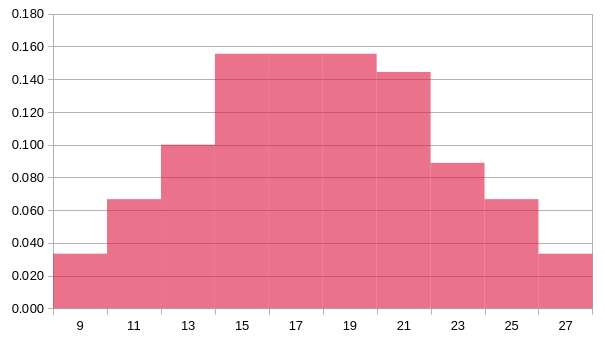
\includegraphics[scale=0.55]{2.png}
\caption{Гистограмма относительных частот}
\end{figure}

\newpage

\noindent Выборочные характеристики:

\begin{align*}
  \overline{X} &= \sum_{i=1}^k x_i^*\tilde{p}_i = \textbf{17.911} & 
  S^2 &= \frac{n}{n-1}\sum_{i=1}^{k}(x_i - \overline{X})^2\tilde{p}_i = \textbf{19.880} \\
  \overline{X^2} &= \sum_{i=1}^k (x_i^*)^2\tilde{p}_i = \textbf{340.467} & 
  S &= \sqrt{S^2} = \textbf{4.459}
\end{align*}
\vspace{5mm}

\noindent Оценка параметров нормального распределения по методу моментов:

\begin{align*}
  \begin{split}
    X \in N(a, \sigma) 
        &\Rightarrow 
        \begin{cases} 
          EX = a \\
          DX = \sigma^2 \\
        \end{cases} \\
        &\Rightarrow
        \begin{cases} 
          m_1(a, \sigma) = EX = a \\
          m_2(a, \sigma) = EX^2 = E^2X + DX = a^2 + \sigma^2
        \end{cases} \\
        &\Rightarrow
        \begin{cases} 
          a = EX \\
          \sigma = \sqrt{EX^2 - a^2}
        \end{cases} \\
        &\Rightarrow
        \begin{cases} 
          a* = \overline{X} = 17.911 \\
          \sigma^* = \sqrt{\overline{X^2} - \overline{X}^2} = 4.434
        \end{cases}
  \end{split}
\end{align*}
\vspace{5mm}

\noindent Оценка параметров равномерного распределения по методу моментов:

\begin{align*}
  \begin{split}
    X \in U(a, b) 
        &\Rightarrow 
        \begin{cases} 
          EX = (a + b) / 2 \\
          DX = (b - a)^2 / 12 \\
        \end{cases} \\
        &\Rightarrow
        \begin{cases} 
          m_1(a, b) = EX = (a + b) / 2 \\
          m_2(a, b) = EX^2 = E^2X + DX = \left(\frac{a + b}{2}\right)^2 + \frac{(b - a)^2}{12}
        \end{cases} \\
        &\Rightarrow
        \begin{cases} 
          a = EX - \sqrt{3(EX^2 - E^2X)} \\
          b = EX + \sqrt{3(EX^2 - E^2X)}
        \end{cases} \\
        &\Rightarrow
        \begin{cases} 
          a^* = \overline{X} - \sqrt{3(\overline{X^2} - \overline{X}^2)} = 10.232 \\
          b^* = \overline{X} + \sqrt{3(\overline{X^2} - \overline{X}^2)} = 25.591
        \end{cases}
  \end{split}
\end{align*}

\begin{figure}[H]
\centering
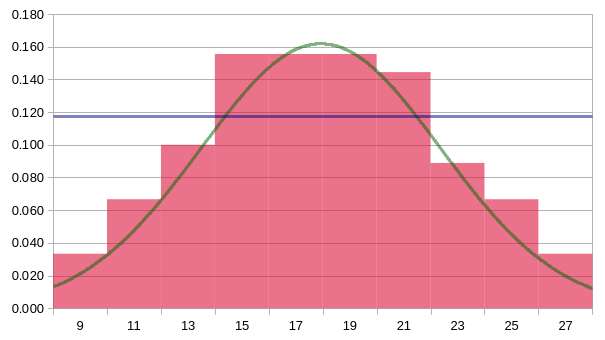
\includegraphics[scale=0.55]{3.png}
\caption{Гистограмма относительных частот}
\end{figure}
\vspace{5mm}

\noindent Оценка параметров нормального распределения по методу максимального правдоподобия:

\begin{align*}
  \begin{split}
    X \in N(a, \sigma)
      &\Rightarrow
      f(x) = \frac{1}{\sigma\sqrt{2\pi}}e^{-\frac{(x-a)^2}{2\sigma^2}} \\
      &\Rightarrow
      \Pi(a, \sigma, X) = \prod_i^n \frac{1}{\sigma\sqrt{2\pi}}e^{-\frac{(x_i-a)^2}{2\sigma^2}} \\
      &\Rightarrow
      \ln\Pi(a, \sigma, X) = \sum_i^n \ln\frac{1}{\sigma\sqrt{2\pi}} 
        + -\ln{e}\sum_i^n \frac{(x_i-a)^2}{2\sigma^2} \\
      &\Rightarrow
      \begin{cases} 
        \frac{\partial{\ln\Pi(a, \sigma, X)}}{\partial{a}}
          = \frac{\overline{X}n}{\sigma^2} - \frac{an}{\sigma^2} = 0 \\
        \frac{\partial{\ln\Pi(a, \sigma, X)}}{\partial{\sigma}}
          = \overline{X^2}n - \sigma^2n - 2a\overline{X}n + a^2n = 0
      \end{cases} \\
      &\Rightarrow
      \begin{cases} 
        a^* = \overline{X} = 17.911 \\
        \sigma^* = \sqrt{\overline{X^2} - \overline{X}^2} = 4.434
      \end{cases}
  \end{split}
\end{align*}
\vspace{5mm}

\newpage

\noindent Оценка параметров равномерного распределения по методу максимального правдоподобия:

\begin{align*}
  \begin{split}
    X \in U(a, b)
      &\Rightarrow
      f(x) = \frac{1}{b - a} \\
      &\Rightarrow
      \Pi(a, b, X) = \prod_i^n \frac{1}{b - a} \\
      &\Rightarrow
      \ln\Pi(a, b, X) = \ln\left( \frac{1}{b - a} \right)^n
        = -n \ln(b - a)\\
      &\Rightarrow
      \begin{cases} 
        \frac{\partial{\ln\Pi(a, b, X)}}{\partial{a}}
          = -\frac{n}{a - b} = 0 \\
        \frac{\partial{\ln\Pi(a, b, X)}}{\partial{b}}
          = -\frac{n}{b - a} = 0
      \end{cases} \\
      &\Rightarrow
      \begin{cases} 
        a^* = min(X) = 8 \\
        b^* = max(X) = 28
      \end{cases}
  \end{split}
\end{align*}
\vspace{5mm}

\noindent Проверка гипотезы о согласии выборки нормальному распределению:

\begin{table}[H]
\centering
\begin{tblr}{
  width=\textwidth, 
  colspec={|c|c|c|X|X|X|X|X|},
  rowspec={|c|cccccccccc|c|}
}
\SetCell{c} $x_i^*$ & \SetCell{c} $n_i$ & \SetCell{c} $x_i^* n_i$ & \SetCell{c} $n_i (x_i^* - \overline{X})^2$ & \SetCell{c} $u_i$  & \SetCell{c} $f(u_i)$  & \SetCell{c} $n_i'$  & \SetCell{c} $R$ \\
9	                  & 3	                & 27	                    & 238.224	                                   & -1.999	            & 0.054	                & 2.186	              & 0.303           \\
11	                & 6	                & 66		                  & 286.581		                                 & -1.550	            & 0.120	                & 4.845	              & 0.276           \\
13	                & 9	                & 117		                  & 217.071		                                 & -1.101	            & 0.217	                & 8.781	              & 0.005           \\
15	                & 14	              & 210		                  & 118.644		                                 & -0.653	            & 0.322	                & 13.014	            & 0.075           \\
17	                & 14	              & 238		                  & 11.622		                                 & -0.204	            & 0.391	                & 15.773	            & 0.199           \\
19	                & 14	              & 266		                  & 16.600		                                 & 0.244	            & 0.387	                & 15.632	            & 0.170           \\
21	                & 13	              & 273		                  & 124.036		                                 & 0.693	            & 0.314	                & 12.669	            & 0.009           \\
23	                & 8	                & 184		                  & 207.174		                                 & 1.141	            & 0.208	                & 8.397	              & 0.019           \\
25	                & 6	                & 150		                  & 301.514		                                 & 1.590	            & 0.113	                & 4.551	              & 0.462           \\
27	                & 3	                & 81		                  & 247.824		                                 & 2.038	            & 0.050	                & 2.017	              & 0.479           \\
$\Sigma$            & 90	              & 1612		                & 1769.289				                           & -                  & -                     & 87.864	            & 1.997
\end{tblr}
\caption{Расчёты}
\end{table}

\begin{gather*}
  k = m - 1 - 2 = 7 \Rightarrow | \alpha = 0.1 | \Rightarrow \chi^2_{cr} = \textbf{12.017} \\[1ex]
  \chi^2_{fn} = \textbf{1.997} \Rightarrow \chi^2_{fn} < \chi^2_{cr} \Rightarrow H_0 - accepted.
\end{gather*}
\vspace{5mm}

\newpage

\noindent Проверка гипотезы о согласии выборки равномерному распределению:

\begin{table}[H]
\centering
\begin{tblr}{
  width=\textwidth, 
  colspec={|X|X|X|X|X|X|},
  rowspec={|c|cccccccccc|c|}
}
\SetCell{c} $x_i$ & \SetCell{c} $x_{i+1}$ & \SetCell{c} $n_i$ & \SetCell{c} $p_i$ & \SetCell{c} $n_i'$  & \SetCell{c} $R$ \\
10.188	          & 10	                  & 3	                & 0.000	            & 0.000	              & 0.000           \\
10	              & 12	                  & 6	                & 0.129	            & 11.654	            & 2.743           \\
12	              & 14	                  & 9	                & 0.129	            & 11.654	            & 0.604           \\
14	              & 16	                  & 14	              & 0.129	            & 11.654	            & 0.472           \\
16	              & 18	                  & 14	              & 0.129	            & 11.654	            & 0.472           \\
18	              & 20	                  & 14	              & 0.129	            & 11.654	            & 0.472           \\
20	              & 22	                  & 13	              & 0.129	            & 11.654	            & 0.155           \\
22	              & 24	                  & 8	                & 0.129	            & 11.654	            & 1.146           \\
24	              & 26	                  & 6	                & 0.129	            & 11.654	            & 2.743           \\
26	              & 25.634	              & 3	                & 0.000	            & 0.000	              & 0.000           \\
$\Sigma$		      & -                     & 90	              & 1.036	            & 93.233	            & 8.809
\end{tblr}
\caption{Расчёты}
\end{table}

\begin{gather*}
  k = m - 1 - 2 = 7 \Rightarrow | \alpha = 0.1 | \Rightarrow \chi^2_{cr} = \textbf{12.017} \\[1ex]
  \chi^2_{fn} = \textbf{8.809} \Rightarrow \chi^2_{fn} < \chi^2_{cr} \Rightarrow H_0 - accepted.
\end{gather*}

\end{document}

